\documentclass[8pt,a4paper,compress]{beamer}
%\documentclass[8pt,a4paper,compress,handout]{beamer}

\usepackage{amsmath, amssymb, amsthm}
\usepackage{enumerate}
\usepackage{framed}
\usepackage{listings}
\usepackage{tikz}
\usetikzlibrary{shapes.gates.logic.US,trees,positioning,arrows,shapes.multipart}
\usepackage{wrapfig}

\usecolortheme{dove}
\useinnertheme{circles}
\beamertemplatenavigationsymbolsempty
\setbeamertemplate{headline}
{
  \leavevmode%
  \hbox{%
  \begin{beamercolorbox}[wd=\paperwidth,ht=6ex]{secsubsec}%
    \raggedright
    \hspace*{1.5em}%
    \normalsize
    \ifx\insertsection\empty\else
      \textbf{\insertsection\text{ }}%
      \ifx\insertsubsection\empty\else
        \textbf{$\bullet$\text{ }\insertsubsection}%
      \fi
    \fi
    \hspace*{2em}%
  \end{beamercolorbox}%
  }%
}
\setbeamerfont{frametitle}{size=\normalsize}
\setbeamertemplate{mini frames}{}
\setbeamertemplate{footline}[page number]

\definecolor{lightgray}{RGB}{240,240,240}
\definecolor{darkgreen}{RGB}{51,102,0}

\title{1.1 Basic Programming Model}
\date{}

\lstset{
  backgroundcolor=\color{lightgray},
  basicstyle=\footnotesize\ttfamily,
  showstringspaces=false,
  commentstyle=\color{darkgreen},
  keywordstyle=\color{blue},
  stringstyle=\color{orange},
}

\begin{document}
\begin{frame}
\vfill
\titlepage
\end{frame}

\begin{frame}
\frametitle{Outline}
\tableofcontents
\end{frame}

\section{Basic Structure of a Java Program}

\begin{frame}[fragile]
\pause

\textbf{Java Program} Either a library of static methods (functions) or a data type definition. To create a Java program (class), we use the following programming constructs:
\begin{itemize}
\item \emph{Primitive Data Types:} define the meaning of terms like integer, real number, and boolean value within a computer program; 
\item \emph{Statements:} allow us to define computation by creating and assigning values to variables, controlling execution flow, or causing side effects; 
\item \emph{Arrays:} allow us to work with multiple values of the same type; 
\item \emph{Static Methods:} allow us to encapsulate and reuse code and to develop programs as a set of independent modules; 
\item \emph{Strings:} sequences of characters used extensively in input and output; 
\item \emph{Input/Output:} sets up communication between programs and the outside world; and 
\item \emph{Data Abstraction} allows us to define our own data types, ie, develop object-oriented programs.
\end{itemize}

\end{frame}

\begin{frame}[fragile]
\pause

Eg: Binary search and whitelisting

\begin{lstlisting}[language=Java]
public class BinarySearch {
    public static int rank(int key, int[] a) {
        int lo = 0;
        int hi = a.length - 1;
        while (lo <= hi) {
            int mid = lo + (hi - lo) / 2;
            if (key < a[mid]) { hi = mid - 1; }
            else if (key > a[mid]) { lo = mid + 1; }
            else { return mid; }
        }
        return -1;
    }

    public static void main(String[] args) {
        In in = new In(args[0]);
        int[] whitelist = in.readAllInts();
        Arrays.sort(whitelist);
        while (!StdIn.isEmpty()) {
            int key = StdIn.readInt();
            if (rank(key, whitelist) == -1) {
                StdOut.println(key);
            }
        }
    }
}
\end{lstlisting}

\begin{lstlisting}[language=bash]
$ java BinarySearch largeW.txt < largeT.txt
499569
984875
...
\end{lstlisting}

\end{frame}

\section{Primitive Data Types and Expressions}
\begin{frame}[fragile]
\pause

\textbf{Data Type} Set of values and a set of operations on those values.

\pause
\smallskip

\textbf{Basic Primitive Types}
\begin{itemize}
\item \lstinline$int$: Integers between $-2^{31}$ and $2^{31}-1$ with arithmetic operations; 
\item \lstinline$double$: Double-precision real numbers (specified by IEEE 754 standard) with arithmetic operations; 
\item \lstinline$boolean$: True and false values with logical operations; and
\item \lstinline$char$: $2^{16}$ (alphanumeric and symbol) characters with arithmetic operations.
\end{itemize}

\pause
\smallskip

\textbf{Expressions} A literal, variable, or a sequence of allowed operations on literals and/or variables that produces a value. The arithmetic operators \lstinline$*$ and \lstinline$/$ (and \lstinline$%$) have higher precedence than \lstinline$+$ and \lstinline$-$; among logical operators, \lstinline$!$ has the highest precedence, followed by \lstinline$&&$ and then \lstinline$||$. Operators of the same precedence are applied left to right. You can use parentheses to override precedence rules.

\pause
\smallskip

\textbf{Type Conversion} Numbers are automatically promoted to a more inclusive type if no information is lost. A cast is a type name in parentheses within an expression, a directive to convert the following value into a value of that type.

\pause
\smallskip

\textbf{Comparisons} Two operands of the same type can be compared using the relational operators \lstinline$==$, \lstinline$!=$, \lstinline$<$, \lstinline$<=$, \lstinline$>$, and \lstinline$>=$. The comparison produces a \lstinline$boolean$ result. The relational operators have higher precedence than logical operators but lower precedence than arithmetic operators.

\pause
\smallskip

\textbf{Other Primitive Types} 
\begin{itemize}
\item 64-bit integers with arithmetic operations (\lstinline$long$); 
\item 16-bit integers with arithmetic operations (\lstinline$short$);
\item 8-bit integers with arithmetic operations (\lstinline$byte$); and
\item 32-bit single-precision real numbers with arithmetic operations (\lstinline$float$).
\end{itemize}

\end{frame}

\section{Statements}
\begin{frame}[fragile]
\pause

Statements define computation by creating and manipulating variables, assigning data-type values to them, and controlling the flow of execution.

\pause
\smallskip

\textbf{Declaration Statement}
Associates a variable name with a type.
\begin{lstlisting}[language=Java]
<type> <name>;
\end{lstlisting}
Initial value for the variable: \lstinline$false$ for Boolean type, \lstinline$0$ for numeric types, and \lstinline$null$ for reference types.

\pause
\smallskip

\textbf{Assignment Statement}
Associates a data-type value with a variable.
\begin{lstlisting}[language=Java]
<name> = <expression>;
\end{lstlisting}

\pause
\smallskip

\textbf{Initialization} Declaration and assignment statements can be combined to provide an initial value for a variable.
\begin{lstlisting}[language=Java]
<type> <name> = <expression>;
\end{lstlisting}
\end{frame}

\begin{frame}[fragile]
\pause
\textbf{Conditionals} Used when different actions are required for different inputs.

\begin{itemize}
\item \textbf{If Statement}
\begin{lstlisting}[language=Java]
if (<boolean expression>) {
    <statements>
}
else if (<boolean expression>) {
    <statements>
}
...
else {
    <statements>
}
\end{lstlisting}

\pause

\item \textbf{Conditional Operator} 
\begin{lstlisting}[language=Java]
String flip = Math.random() < 0.5 ? "Heads" : "Tails";
\end{lstlisting}

\pause

\item \textbf{Switch Statement} 
\begin{lstlisting}[language=Java]
switch (day) {
    case 0:
        System.out.println("Sunday");
        break;
    case 1:
        System.out.println("Monday");
        break;
    ...
    case 6:
        System.out.println("Saturday");
        break;
    default:
        System.out.println("Error!");
}
\end{lstlisting}

\end{itemize}
\end{frame}

\begin{frame}[fragile]
\pause
\textbf{Loops} Used for repetitive computations.

\pause
\smallskip

\begin{itemize}
\item \textbf{While Statement}
\begin{lstlisting}[language=Java]
while (<boolean expression>) {
    <statements>
}
\end{lstlisting}

\pause

\item \textbf{For Statement} 
\begin{lstlisting}[language=Java]
for (<initialize>; <boolean expression>; <increment>) {
    <statements>
}
\end{lstlisting}

\pause
\item \textbf{Do-while Statement} 
\begin{lstlisting}[language=Java]
do {
    <statements>
} while (<boolean expression>);
\end{lstlisting}

\pause

\item \textbf{Break Statement} Immediately exits a loop without letting it to run to completion. 

\pause

\item \textbf{Continue Statement} Skips to next iteration of a loop.
\end{itemize}

\pause
\smallskip

\textbf{Compound Assignment Idiom} Shorthand notation for modifying the value of a variable. Eg, \lstinline$i = i + 1;$, \lstinline$i++;$, and \lstinline$i += 1;$ are equivalent statements, and so are \lstinline$v *= 2;$, \lstinline$v = 2 * v;$, and \lstinline$v += v;$.

\pause
\smallskip

\textbf{Scope of a Variable} Part of the program where it is defined;  statements that follow the declaration in the same block (marked by \lstinline${...}$) as the declaration.
\end{frame}

\section{Arrays}
\begin{frame}[fragile]
\pause

An array stores a sequence of values that are all of the same type. Making an array in a Java program involves three steps:
\begin{itemize}
\item Declaring the array name and type; 
\item Creating the array; and
\item Initializing the array values.
\end{itemize}
\begin{lstlisting}[language=Java]
double[] a;
a = new double[N];
for (int i = 0; i < N; i++) {
    a[i] = 0.0;
}
\end{lstlisting}

\pause
\smallskip
\textbf{Default Array Initialization} An array when declared is initialized to \lstinline$null$; once created, each element is initialized to a default value based on the type of the array.

\pause
\smallskip
\textbf{Initializing Declaration}
\begin{lstlisting}[language=Java]
int[] a = {1, 1, 2, 3, 5, 8, 13, 21, 34, 55};
String[] b = {"Sun", "Mon", "Tue", "Wed", "Thu", "Fri", "Sat"};
\end{lstlisting}

\pause
\smallskip
\textbf{Using an Array} After declaring and creating an array, you can refer to any individual value by enclosing an integer index (zero based) in square brackets after the array name. A program can refer to the length of an array \lstinline$a[]$ as \lstinline$a.length$. Eg, the following code reverses the array \lstinline$a$ in place:
\begin{lstlisting}[language=Java]
int N = a.length;
for (int i = 0; i < N / 2; i++) {
    double temp = a[i];
    a[i] = a[N - 1 -i];
    a[N - i - 1] = temp;
}
\end{lstlisting}
\end{frame}

\begin{frame}[fragile]
\pause

\textbf{Aliasing} If we assign one array name to another, then both refer to the same array.

\pause
\smallskip

\textbf{Two-dimensional Arrays} A two-dimensional array in Java is an array of one-dimensional arrays. A two-dimensional array may be ragged. We mostly work with two-dimensional arrays that are arrays of $m$ rows, each an array of length $n$ (ie, $n$ columns). Eg, the following code multiplies two matrices $A_{m\times p}$ and $B_{p\times n}$ represented by arrays \lstinline$A$ and \lstinline$B$ respectively and stores the resulting matrix $C_{m\times n}$ in array \lstinline$C$; recall that $$C_{ij}=\sum_{k=1}^{p} A_{ik}B_{kj}.$$
\begin{lstlisting}[language=Java]
int m = A.length;
int p = B.length;
int n = B[0].length;
double[][] C = new double[m][n];
for (int i = 0; i < m; i++) {
    for (int j = 0; j < n; j++) {
        for (int k = 0; k < p; k++) {
            C[i][j] += A[i][k] * B[k][j];
        }
    }
}
\end{lstlisting}

\end{frame}

\section{Static Methods}
\begin{frame}[fragile]
\pause

\textbf{Defining a Static Method} A method encapsulates a computation defined as a sequence of statements. A static method is composed of the keywords \lstinline$public static$ followed by a return type (or \lstinline$void$), the signature (method name and a sequence of arguments, each with a declared type), and a \emph{body} (a statement block: a sequence of statements enclosed by curly brackets). Eg, the following static method tests if the argument \lstinline$N$ is prime and returns \lstinline$true$ if it is and \lstinline$false$ otherwise.

\begin{lstlisting}[language=Java]
public static boolean isPrime(int N) {
    if (N < 2) {
        return false;
    }
    for (int i = 2; i * i <= N; i++) {
        if (N % i == 0) {
            return false;
        }
    }
    return true;
}
\end{lstlisting}

\pause
\smallskip

\textbf{Invoking a Static Method} A \emph{call} on a static method is its name followed by expressions that specify argument values in parentheses, separated by commas. When the method call is part of an expression, the method computes a value and that value is used in place of the call in the expression. Eg, call on \lstinline$rank()$ in \lstinline$BinarySearch$. A method call followed by a semicolon is a statement that generally causes side effects. Eg, the statement \lstinline$Arrays.sort();$ in \lstinline$BinarySearch.main()$.

\end{frame}

\begin{frame}[fragile]
\pause

\textbf{Properties of Methods}
\begin{itemize}
\item Arguments are passed by value; 
\item Method names can be overloaded; 
\item A method has a single return value but may have multiple return statements; and
\item A method can have side effects.
\end{itemize}

\pause
\smallskip

\textbf{Recursion} A method that calls itself. Important rules in developing recursive methods:
\begin{itemize}
\item The recursion has a \emph{base case}; 
\item Recursive calls must address subproblems that are \emph{smaller} in some sense; and
\item Recursive calls should not address subproblems that \emph{overlap}.
\end{itemize}

\pause

Eg: (good recursive solution) computing $N!$

\begin{lstlisting}[language=Java]
public static int factorial(int N) {
    return (N == 0) ? 1 : N * factorial(N - 1); 
}
\end{lstlisting}

\pause

Eg: (bad recursive solution) computing the $N$th Fibonacci number
\begin{lstlisting}[language=Java]
public static int fibonacci(int N) {
    return (N == 0 || N == 1) ? 1 : fibonacci(N - 1) + fibonacci(N - 2); 
}
\end{lstlisting}

\pause
\smallskip

\textbf{Unit Testing} A best practice in Java programming is to include a \lstinline$main()$ method (aka development or test client) in every library of static methods that tests the methods in the library.

\end{frame}

\begin{frame}[fragile]
\pause
\textbf{External Libraries} We use static methods from four different kinds of libraries:
\begin{itemize}
\item The standard system libraries \lstinline$java.lang.*$; 
\item Imported system libraries such as \lstinline$java.util.Arrays$; 
\item Other libraries in the text. Eg, another program can use \lstinline$BinarySearch.rank()$; and
\item The standard libraries \lstinline$Std*$ from the text.
\end{itemize}
\end{frame}

\section{APIs}
\begin{frame}[fragile]
\pause
\textbf{Application Programming Interface (API)} Lists the library name and the return type, signatures, and short descriptions of each of the methods. 

\pause
\smallskip

\textbf{Client} A program that calls a method in another library.

\pause
\smallskip

\textbf{Implementation} The Java code that implements the methods in an API.

\pause
\smallskip

\textbf{Java Libraries}
\begin{itemize}
\item Excerpts from Java API for mathematics (\lstinline$java.lang.Math$)
\begin{lstlisting}[language=Java]
public class Math

    double abs(double a)           // absolute value of a
    double max(double a, double b) // maximum of a and b
    double min(double a, double b) // minimum of a and b
    double sin(double theta)       // sine function
    double cos(double theta)       // cosine function
    double tan(double theta)       // tangent function
    double random()                // random number in [0, 1)
    double E                       // value of e (constant)
    double PI                      // value of pi (constant)
\end{lstlisting}

\item Excerpt from Java's Arrays API (\lstinline$java.util.Arrays$)
\begin{lstlisting}[language=Java]
public class Arrays

    void sort(int[] a) // put the array in increasing order
\end{lstlisting}
\end{itemize}

\end{frame}

\begin{frame}[fragile]
\pause

\textbf{Standard Libraries from the Text}
\begin{itemize}
\item Excerpts from the API for random numbers (\lstinline$StdRandom$)
\begin{lstlisting}[language=Java]
public class StdRandom

    void initialize(long seed)           // initialize
    double random()                      // real between 0 and 1
    int uniform(int N)                   // integer between 0 and N-1
    int uniform(int lo, int hi)          // integer between lo and hi-1
    double uniform(double lo, double hi) // real between lo and hi
    boolean bernoulli(double p)          // true with probability p
    double gaussian()                    // normal, mean 0, std dev 1
    double gaussian(double m, double s)  // normal, mean m, std dev s
    int discrete(double[] a)             // i with probability a[i]
    void shuffle(double[] a)             // randomly shuffle the array a[]
\end{lstlisting}

\item Excerpt from the API for data analysis (\lstinline$StdStats$)
\begin{lstlisting}[language=Java]
public class StdStats

    double max(double[] a)    // largest value
    double min(double[] a)    // smallest value
    double mean(double[] a)   // average
    double var(double[] a)    // sample variance
    double stddev(double[] a) // sample standard deviation
    double median(double[] a) // median
\end{lstlisting}
\end{itemize}

\pause
\smallskip

\textbf{Your Own Libraries} Consider every program that you write as a library implementation, for possible reuse in the future.
\begin{itemize}
\item Write code for the client; 
\item Design an API for a library of static methods; and
\item Develop an implementation of the API, with a \lstinline$main()$ method that tests the methods independent of the client.
\end{itemize}
\end{frame}

\section{Strings}
\begin{frame}[fragile]
\pause

A \lstinline$String$ is a sequence of characters (\lstinline$char$ values). A \lstinline$String$ literal is a sequence of characters within double quotes, such as \lstinline$"Hello, World"$. 

\pause
\smallskip

\textbf{Concatenation} The result of concatenating two \lstinline$String$ values using the \lstinline$+$ operator is a single \lstinline$String$ value, the first string followed by the second.

\pause
\smallskip

\textbf{Strings to Primitive Type Values for Command-line Arguments} Use Java library methods such as \lstinline$Integer.parseInt()$, \lstinline$Double.parseDouble()$, and so on. Eg, \lstinline$Integer.parseInt("42")$ converts the string \lstinline$"42"$ to the integer \lstinline$42$.

\pause
\smallskip


\textbf{Primitive Type Values to Strings for Output} Whenever we use the \lstinline$+$ operator with \lstinline$String$ as one of its operands, Java automatically converts the other to a \lstinline$String$, producing a string formed from the characters of the first operand followed by the characters of the second operand. Eg, The following code snippet 

\begin{lstlisting}[language=Java]
String a = "1234";
int b = 99;
String c = a + b;
int d = 1333;
System.out.println(c);
System.out.println(a + " + " + b + " = " + d);
\end{lstlisting}

produces the output
\begin{lstlisting}[language=bash]
123499
1234 + 99 = 1333 
\end{lstlisting}

\end{frame}

\section{Input and Output}
\begin{frame}[fragile]
\pause

\textbf{Bird's-eye View of a Java Program}
\begin{center}
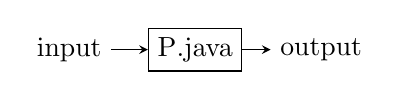
\begin{tikzpicture}
\begin{scope}[->,xshift=-7.5cm,yshift=-5cm,thin,
	   node distance=1.6cm,on grid,>=stealth,
  	   block1/.style={rectangle,draw,align=center},
	   block2/.style={rectangle,align=center}]
\node [block2] (1) {input};
\node [block1] (2) [right=of 1] {\lstinline$P.java$};
\node [block2] (3) [right=of 2] {output};
\path (1) edge node [above] {} (2);
\path (2) edge node [above] {} (3);
\end{scope}
\end{tikzpicture}
\end{center}
\begin{itemize}
\item Input types: command-line arguments, standard input, file input.
\item Output types: standard output, file output, graphical output.
\end{itemize}

\pause
\smallskip

\textbf{Standard Output}

\begin{lstlisting}[language=Java]
public class StdOut

    void print(String s)       // print s
    void println(String s)     // print s, followed by a newline
    void println()             // print a newline
    void printf(String f, ...) // formatted print
\end{lstlisting}

\pause
\smallskip

\textbf{Sample \lstinline$StdOut$ Client}

\begin{lstlisting}[language=Java]
public class RandomSeq {
    public static void main(String[] args) { 
        int N = Integer.parseInt(args[0]);
        double lo = Double.parseDouble(args[1]);
        double hi = Double.parseDouble(args[2]);
        for (int i = 0; i < N; i++) {
            double x = StdRandom.uniform(lo, hi);
            StdOut.printf("%.2f\n", x);
        }
    }
}
\end{lstlisting}

\pause

\begin{lstlisting}[language=bash]
$ java RandomSeq 2 100.0 200.0
193.12
190.79
\end{lstlisting}
\end{frame}

\begin{frame}[fragile]
\pause

\textbf{Standard Input}

\begin{lstlisting}[language=Java]
public class StdIn

    boolean isEmpty()     // true if no more values, false otherwise
    int readInt()         // read a value of type int
    double readDouble()   // read a value of type double
    float readFloat()     // read a value of type float
    long readLong()       // read a value of type long
    boolean readBoolean() // read a value of type boolean
    char readChar()       // read a value of type char
    byte readByte()       // read a value of type byte
    String readString()   // read a value of type String
    boolean hasNextLine() // is there another line in the input stream?
    String readLine()     // read the rest of the line
    String readAll()      // read the rest of the input stream
\end{lstlisting}

\pause
\smallskip

\textbf{Sample \lstinline$StdIn$ Client}

\begin{lstlisting}[language=Java]
public class Average { 
    public static void main(String[] args) { 
        int count = 0; 
        double sum = 0.0;
        while (!StdIn.isEmpty()) {
            double value = StdIn.readDouble();
            sum += value;
            count++;
        }
        double average = sum / count;
        StdOut.println("Average is " + average);
    }
}
\end{lstlisting}
\end{frame}

\begin{frame}[fragile]
\pause

\begin{lstlisting}[language=bash]
$ java Average
1.23456
2.34567
3.45678
4.56789
<ctrl-d>
Average is 2.901225
\end{lstlisting}

\pause
\smallskip

\textbf{Redirection and Piping}

\begin{lstlisting}[language=bash]
$ java RandomSeq 1000 100.0 200.0 > data.txt
$ head -5 data.txt
155.83
191.65
197.83
191.90
111.84
\end{lstlisting}

\begin{lstlisting}[language=bash]
$ java Average < data.txt
Average is 149.1812199999999
\end{lstlisting}

\begin{lstlisting}[language=bash]
$ java RandomSeq 1000 100.0 200.0 | java Average
Average is 150.0588699999999
\end{lstlisting}

\end{frame}

\begin{frame}[fragile]
\pause

\textbf{File Input and Output}

\begin{lstlisting}[language=Java]
public class In

    int[] readInts(String name)       // read int values
    double[] readDoubles(String name) // read double values
    String[] readStrings(String name) // read String values
\end{lstlisting}

\begin{lstlisting}[language=Java]
public class Out

    void write(int[] a, String name)    // write int values
    void write(double[] a, String name) // write double values
    void write(String[] a, String name) // write String values
\end{lstlisting}

\pause
\smallskip

\textbf{Sample \lstinline$In$/\lstinline$Out$ Client}

\begin{lstlisting}[language=Java]
public class Cat { 
   public static void main(String[] args) { 
        Out out = new Out(args[args.length - 1]);
        for (int i = 0; i < args.length - 1; i++) {
            In in = new In(args[i]);
            String s = in.readAll();
            out.println(s);
            in.close();
        }
        out.close();
    }
}
\end{lstlisting}

\pause

\begin{lstlisting}[language=bash]
$ more A.txt
To be, or not to be, that is the question
$ java Cat A.txt B.txt
$ more B.txt
To be, or not to be, that is the question.

\end{lstlisting}
\end{frame}

\begin{frame}[fragile]
\pause

\textbf{Standard Drawing (Drawing Methods)}

\begin{lstlisting}[language=Java]
public class StdDraw

    void line(double x0, double y0, double x1, double y1)
    void point(double x, double y)
    void text(double x, double y, String s)
    void circle(double x, double y, double r)
    void filledCircle(double x, double y, double r)
    void ellipse(double x, double y, double rw, double rh)
    void filledEllipse(double x, double y, double rw, double rh)
    void square(double x, double y, double r)
    void filledSquare(double x, double y, double r)
    void rectangle(double x, double y, double rw, double rh)
    void filledRectangle(double x, double y, double rw, double rh)
    void polygon(double[] x, double[] y)
    void filledPolygon(double[] x, double[] y)
\end{lstlisting}

\textbf{Standard Drawing (Control Methods)}

\begin{lstlisting}[language=Java]
public class StdDraw

    void setXscale(double x0, double x1) // reset x range to (x 0 , x 1 )
    void setYscale(double y0, double y1) // reset y range to (y 0 , y 1 )
    void setPenRadius(double r)          // set pen radius to r
    void setPenColor(Color c)            // set pen color to c
    void setFont(Font f)                 // set text font to f
    void setCanvasSize(int w, int h)     // set canvas to w-by-h window
    void clear(Color c)                  // clear the canvas; color it c
    void show(int dt)                    // show all; pause dt milliseconds
\end{lstlisting}
\end{frame}

\begin{frame}[fragile]
\pause

\textbf{Sample \lstinline$StdDraw$ Client}

\begin{lstlisting}[language=Java]
public class Functions {
    public static void main(String[] args) {
        int N = 100;
        StdDraw.setXscale(0, N);
        StdDraw.setYscale(0, N * N);
        StdDraw.setPenRadius(.01);
        for (int i = 1; i <= N; i++) {
            StdDraw.point(i, i);
            StdDraw.point(i, i * i);
            StdDraw.point(i, i * Math.log(i));
        }
    }	
}
\end{lstlisting}

\pause

\begin{lstlisting}[language=bash]
$ java Functions
\end{lstlisting}

\includegraphics[scale=0.2]{./figures/functions.pdf}

\end{frame}

\section{Binary Search}
\begin{frame}[fragile]
\pause

Implemented in \lstinline$BinarySearch.java$ as a static method \lstinline$rank()$ that takes an integer key and a sorted array of values as input and returns the index of the key if it is present in the array, \lstinline$-1$ otherwise.

\pause
\smallskip

Successful search for the key 23:

\begin{center}
\includegraphics[scale=0.4]{./figures/bs1.pdf}
\end{center}
\end{frame}

\begin{frame}[fragile]
\pause

Unsuccessful search for the key 50:

\begin{center}
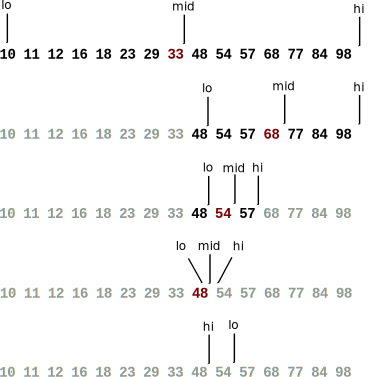
\includegraphics[scale=0.4]{./figures/bs2.pdf}
\end{center}
\end{frame}

\begin{frame}[fragile]
\pause

\textbf{Whitelist Client} The client (\lstinline$BinarySearch.main()$ method) reads integers (eg, customers account numbers) from the file named on the command line and prints any integers (eg, account numbers associated with transactions) on standard input that do not appear in the file. 

\pause
\smallskip

\textbf{Binary Search and Whitelisting}

\begin{lstlisting}[language=Java]
public class BinarySearch {
    public static int rank(int key, int[] a) {
        int lo = 0;
        int hi = a.length - 1;
        while (lo <= hi) {
            int mid = lo + (hi - lo) / 2;
            if (key < a[mid]) { hi = mid - 1; }
            else if (key > a[mid]) { lo = mid + 1; }
            else { return mid; }
        }
        return -1;
    }

    public static void main(String[] args) {
        In in = new In(args[0]);
        int[] whitelist = in.readAllInts();
        Arrays.sort(whitelist);
        while (!StdIn.isEmpty()) {
            int key = StdIn.readInt();
            if (rank(key, whitelist) == -1) {
                StdOut.println(key);
            }
        }
    }
}
\end{lstlisting}
\end{frame}

\begin{frame}[fragile]
\pause

\begin{lstlisting}[language=bash]
tinyW.txt tinyT.txt
   84        23
   48        50
   68        10
   10        99
   18        18
   98        23
   12        98
   23        84
   54        11
   57        10
   48        48
   33        77
   16        13
   77        54
   11        98
   29        77
             77
             68
\end{lstlisting}

\pause

\begin{lstlisting}[language=bash]
$ java BinarySearch tinyW.txt < tinyT.txt
50
99
13
\end{lstlisting}

\pause
\smallskip

\textbf{Performance} Solving the whitelist problem for a large number of inputs is not feasible without efficient algorithms such as binary search and merge sort. The following simpler implementation for \lstinline$rank()$ will just not scale.

\begin{lstlisting}[language=Java]
public static int rank(int key, int[] a) {
    for (int i = 0; i < a.length; i++) {
        if (a[i] == key) { return i; }
    }
    return -1;
}
\end{lstlisting}
\end{frame}

\begin{frame}[fragile]
\pause

\textbf{Recursive Implementation of \lstinline$BinarySearch.rank()$}

\begin{lstlisting}[language=Java]
public static int rank(int key, int[] a) { 
    return rank(key, a, 0, a.length - 1);
}

private static int rank(int key, int[] a, int lo, int hi) {
    if (lo > hi) {
        return -1;
    }
    int mid = lo + (hi - lo) / 2;
    if (key < a[mid]) {
        return rank(key, a, lo, mid - 1);
    }
    else if (key > a[mid]) {
        return rank(key, a, mid + 1, hi);
    }
    else {
        return mid;
    }
}
\end{lstlisting}

\end{frame}
\end{document}
